\documentclass[9pt,a4paper]{extarticle}
\usepackage[margin=1.0cm,top=0.85cm,bottom=0.8cm]{geometry}
\usepackage{amsmath}
\usepackage{booktabs}
\usepackage{array}
\usepackage{tabularx}
\usepackage[table]{xcolor}
\usepackage{enumitem}
\usepackage[hidelinks]{hyperref}
\usepackage{titlesec}
\usepackage{tikz}
\usetikzlibrary{arrows.meta}
\usepackage{pgfplots}
\pgfplotsset{compat=1.17}
\usepgfplotslibrary{groupplots}

\setlist{nosep,leftmargin=1.0em}
\setlength{\parskip}{1pt}
\setlength{\parindent}{0pt}
\titleformat{\section}{\large\bfseries}{\thesection}{0.5em}{}
\titlespacing*{\section}{0pt}{3pt}{1pt}
\titleformat{\subsection}{\normalsize\bfseries}{}{0pt}{}
\titlespacing*{\subsection}{0pt}{2.5pt}{0.5pt}
\newcommand{\ci}[2]{[#1,\,#2]}
\newcommand{\term}[1]{\textbf{#1}}
\renewcommand{\arraystretch}{1.03}
\pagestyle{empty}

\begin{document}
{\centering
{\Large\textbf{How Fast Does a News Recommender Go Stale?}}\\[1pt]
{\footnotesize CS4.406 (IRE) term project, IIIT Hyderabad, Monsoon 2026\quad Noel Alex Jacob (2025201085), Emil Joji (2025201040), Kspsvln Siddardha Kumar Kavuri (2025201061)}\par}

\section{What we proposed, and the short answer}
A news article lives for hours, not months. A recommender trained once and then left alone (\term{frozen}) behaves as if the world had not moved. Our proposal asked: \textbf{RQ1} how fast does quality fall, and in what shape (linear, cliff or plateau)? \textbf{RQ2} which of three separable signals (word matching, meaning matching, co-click history) falls first, and why? \textbf{RQ3} how often must the model be rebuilt, as a cost--quality trade-off? We also recorded what we expected: co-click history to fall most (cold start), meaning matching least (by construction), and a flat curve to be a valid answer. Every number carries a 95\% bootstrap interval in brackets and its $n$.
\begin{itemize}
\item \textbf{RQ1, two time scales.} Co-click history can score 79.4\% \ci{79.2}{79.6} of clicks one hour after the freeze and 0.93\% \ci{0.88}{0.97} after a day; text signals fall gradually, word matching losing 9.7\% \ci{7.8}{11.6} of its score in a week (old profile), with no cliff.
\item \textbf{RQ2, as expected.} Co-click history falls first (cold start), meaning matching last, word matching between them; text falls only through the old reader profile, while the proposed vocabulary and embedding-drift mechanisms are real but small.
\item \textbf{RQ3, it depends on the signal and the site.} Text with a live profile need not be rebuilt within 14 days; with an old profile a weekly rebuild stays within 3.9\% of a daily one; click-based signals need hours on a fast site and days on a slow one.
\item \textbf{Added while testing.} ``Newest first'' wins only on the 48-hour pool; on real slates it is no better than random (AUC 0.5026 \ci{0.5010}{0.5042} against 0.4991 \ci{0.4973}{0.5008}). A live count of the last hour's clicks beats it on both, by 0.149 \ci{0.147}{0.151} MRR on the pool and 0.168 \ci{0.166}{0.170} on real slates, but ages in minutes only on the pool.
\end{itemize}

\section{How we measured it, and what we added while testing}
\textbf{One click, one ranking.} A scorer ranks the other articles for a real click and we note where the clicked one lands: \term{MRR} averages $1/\text{rank}$, \term{AUC} is the chance of outranking a random other article (0.5 = random). The others are the \term{pool} (every article published in the 48 hours before the click; the main test) or the \term{real slate} (the articles the site showed that reader in that visit, median 8 to 9; EB-NeRD, 25--31 May 2023, $n=136{,}674$); a pool number is never compared with a slate number. \textbf{Freezing and waiting.} A scorer is fitted on the 7 days of clicks ending on a \term{fit date} and scores clicks \term{lag} days later; the \term{control} is the same scorer rebuilt the day before, and \textbf{decay = control MRR $-$ frozen MRR} on the same clicks. With an \term{old profile} (regime A) the reader's history is frozen at the fit date; with a \term{live profile} (regime B) it is their last 50 clicks. \textbf{Scorers.} In the proposal: word matching (BM25), meaning matching (frozen multilingual MiniLM), co-click history. Added while testing: newest first, most clicked, genre, live trending (all readers' clicks in the last hour; nothing fitted), random order. \textbf{Rules.} Re-reads (15\% of clicks) are dropped; an article a scorer cannot score goes to the bottom in random order, so we report \term{coverage}. \textbf{Data.} EB-NeRD (Danish) is main: 14 fit dates (10--23 May 2023), lags 1 to 13, 20{,}000 clicks a day; NPR and Adressa are second sites.
\textbf{Added while testing, and why.} A control rebuilt the day before (weekdays differ, so a raw score cannot show decay); an old and a live profile (little else is frozen in a text model); newest first and random order as references; an hourly axis (the fall happens within hours); genre and live trending (newest first dominated, and no live click signal had been tried); real slates (the proposal's own evaluation); NPR, Adressa and one-at-a-time checks (EB-NeRD is main as public Adressa has titles only; do the findings travel?).

\section{Results, by research question}
\subsection{RQ1. How fast, and in what shape?}
\textbf{Why it happens (no model).} Six hours after a freeze, the share of the next clicks that go to articles published after it is 90.8\% \ci{88.5}{92.5} on EB-NeRD, 48.5\% \ci{45.4}{51.5} on Adressa and 15.5\% \ci{11.3}{20.1} on NPR ($n$ = 3.46 M, 1.26 M, 72{,}136). From the article's side, its click rate halves 1.74 h \ci{1.72}{1.77} after the peak (3{,}021 articles, 70.6 M clicks).
\textbf{Click-based signals.} Co-click history can score 79.4\% \ci{79.2}{79.6} of clicks after 1 hour and 0.93\% \ci{0.88}{0.97} after 24 hours; this coverage halves every 3.02 h \ci{3.00}{3.03} (40 hourly cells of up to 5{,}000 clicks).
\textbf{Text signals.} With an old profile, the share of the lag-1 score lost at lag 7 and lag 13 is: word 9.7\% \ci{7.8}{11.6} and 18.9\% \ci{15.2}{22.7}; genre 4.3\% \ci{3.1}{5.4} and 16.9\% \ci{14.6}{19.1}; meaning 3.0\% \ci{1.4}{4.4} and 5.4\% \ci{1.8}{8.9} ($n=135{,}583$ and 34{,}479). The fall is gradual, close to linear for word and meaning, with no cliff or plateau by lag 13; genre speeds up.

\begin{figure}[h]
\centering
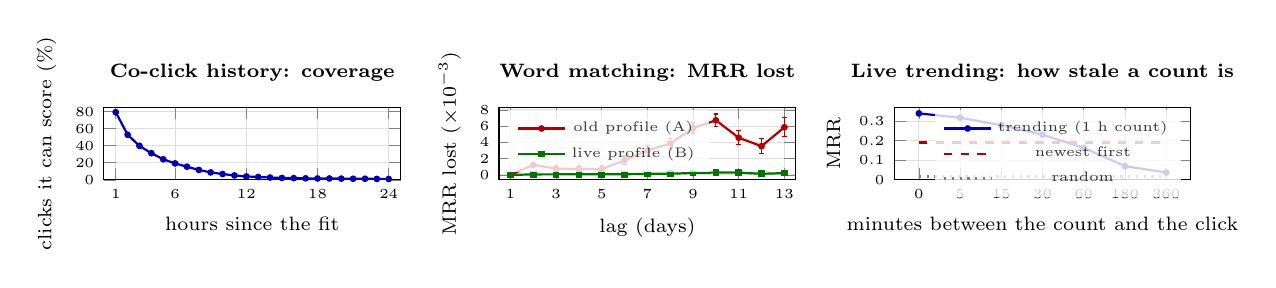
\begin{tikzpicture}
\begin{groupplot}[group style={group size=3 by 1, horizontal sep=1.25cm}, width=5.35cm, height=2.5cm, tick label style={font=\tiny}, label style={font=\scriptsize}, title style={font=\scriptsize\bfseries, align=center}, grid=major, grid style={gray!25}]
\nextgroupplot[title={Co-click history: coverage}, xlabel={hours since the fit}, ylabel={clicks it can score (\%)}, xmin=0, xmax=25, ymin=0, ymax=85, xtick={1,6,12,18,24}]
\addplot[blue!70!black, thick, mark=*, mark size=0.8pt] coordinates {(1,79.39) (2,52.96) (3,39.85) (4,31.23) (5,24.11) (6,19.24) (7,15.37) (8,11.57) (9,8.67) (10,6.76) (11,5.12) (12,3.92) (13,3.27) (14,2.63) (15,2.11) (16,1.97) (17,1.71) (18,1.55) (19,1.55) (20,1.33) (21,1.18) (22,1.21) (23,1.02) (24,0.93)};
\nextgroupplot[title={Word matching: MRR lost}, xlabel={lag (days)}, ylabel={MRR lost ($\times 10^{-3}$)}, xmin=0.5, xmax=13.5, ymin=-0.6, legend style={font=\tiny, at={(0.03,0.97)}, anchor=north west, draw=none, fill=white, fill opacity=0.8}, xtick={1,3,5,7,9,11,13}]
\addplot[red!70!black, thick, mark=*, mark size=0.8pt, error bars/.cd, y dir=both, y explicit] coordinates {(1,0.0000) +- (0,0.0000) (2,1.2490) +- (0,0.2970) (3,0.7750) +- (0,0.3840) (4,0.7320) +- (0,0.4420) (5,0.7010) +- (0,0.4500) (6,1.8230) +- (0,0.5030) (7,3.0060) +- (0,0.6040) (8,3.8750) +- (0,0.5970) (9,5.7750) +- (0,0.6630) (10,6.7370) +- (0,0.7690) (11,4.5880) +- (0,0.8450) (12,3.5400) +- (0,0.9380) (13,5.8710) +- (0,1.1850)};
\addplot[green!45!black, thick, mark=square*, mark size=0.8pt, error bars/.cd, y dir=both, y explicit] coordinates {(1,0.0000) +- (0,0.0000) (2,0.0620) +- (0,0.0310) (3,0.0690) +- (0,0.0370) (4,0.0760) +- (0,0.0420) (5,0.0710) +- (0,0.0440) (6,0.0820) +- (0,0.0520) (7,0.1300) +- (0,0.0620) (8,0.1410) +- (0,0.0710) (9,0.2460) +- (0,0.0880) (10,0.2900) +- (0,0.1060) (11,0.2900) +- (0,0.1300) (12,0.1390) +- (0,0.1240) (13,0.2230) +- (0,0.1830)};
\legend{old profile (A), live profile (B)}
\nextgroupplot[title={Live trending: how stale a count is}, xlabel={minutes between the count and the click}, ylabel={MRR}, symbolic x coords={0,5,15,30,60,180,360}, xtick=data, xticklabel style={font=\tiny}, ymin=0, ymax=0.37, legend style={font=\tiny, at={(0.97,0.97)}, anchor=north east, draw=none, fill=white, fill opacity=0.8}]
\addplot[blue!70!black, thick, mark=*, mark size=0.8pt] coordinates {(0,0.3396) (5,0.3179) (15,0.2790) (30,0.2308) (60,0.1632) (180,0.0699) (360,0.0371)};
\addplot[red!70!black, dashed, thick] coordinates {(0,0.1905) (5,0.1905) (15,0.1905) (30,0.1905) (60,0.1905) (180,0.1905) (360,0.1905)};
\addplot[gray, dotted, thick] coordinates {(0,0.0172) (5,0.0172) (15,0.0172) (30,0.0172) (60,0.0172) (180,0.0172) (360,0.0172)};
\legend{trending (1 h count), newest first, random}
\end{groupplot}
\end{tikzpicture}\\[-2pt]
{\footnotesize \textbf{Figure 1.} EB-NeRD. Left: co-click history loses its reach within hours. Middle: word matching loses score only with an old profile (bars: 95\% intervals). Right: a one-hour trending count that ended 30 minutes before the click still beats newest first; one that ended an hour before does not ($n=236{,}387$).}
\end{figure}
\vspace{-11pt}
\subsection{RQ2. Which signal falls first, and why?}
The order is as we expected: co-click history, then word matching, then genre, then meaning matching (shares above). The proposal's three diagnostics were measured as the difference between the frozen model and its control on the same clicks: the share of clicks co-click history cannot score (cold start); the \term{unseen-term share} for word matching (distinct words of the clicked article that no article published before the fit end contains); the \term{embedding drift} for meaning matching (cosine to the centroid of the previous week's articles). We added the \term{similarity gap} (how much more the clicked article resembles the reader's profile than the average pool article does).
\begin{center}\footnotesize
\setlength{\tabcolsep}{3pt}
\begin{tabular}{@{}l>{\raggedright\arraybackslash}p{10.9cm}>{\raggedright\arraybackslash}p{4.8cm}@{}}
\toprule
\textbf{Signal} & \textbf{Old profile (A)} & \textbf{Live profile (B)}\\
\midrule
Co-click history & unscorable share of clicks: 88.0\% \ci{87.8}{88.1} at lag 1, 99.6\% \ci{99.58}{99.63} at lag 2, 100\% from lag 3 (scorable 0.93\% \ci{0.88}{0.97} at 24 h) & same coverage (12\% at lag 1, none at lag 7): a live profile cannot score a new article\\
Word matching & unseen terms, extra over the control: 0.0028 \ci{0.0027}{0.0029} at lag 2, 0.0033 \ci{0.0032}{0.0034} at lag 7, 0.0036 \ci{0.0034}{0.0037} at lag 13; gap falls by 0.0205 \ci{0.0167}{0.0245} by lag 7 ($n=116{,}893$); MRR lost 0.0030 \ci{0.0024}{0.0036} ($n=135{,}583$) & gap falls by 0.0022 \ci{0.0020}{0.0024} ($n=135{,}233$); MRR lost 0.00013 \ci{0.00007}{0.00019}\\
Meaning matching & embedding drift: 0.0012 \ci{0.0012}{0.0013} at lag 2, 0.0079 \ci{0.0078}{0.0080} at lag 7, 0.0109 \ci{0.0107}{0.0111} at lag 13 (cosine 0.3422 at lag 1); gap falls by 0.0155 \ci{0.0128}{0.0183} ($n=116{,}893$); MRR lost 0.0007 \ci{0.0003}{0.0011} & exactly 0: the article vectors never change, so the drift costs nothing\\
\bottomrule
\end{tabular}
\end{center}
\textbf{Reading the diagnostics.} Both proposed mechanisms exist but are small, and neither explains the loss. Unseen words appear at once (+0.0028 by lag 2) and then barely rise, while the word-matching loss keeps rising; with a live profile, where the vocabulary is the only frozen part, the loss is 0.00013 \ci{0.00007}{0.00019} by lag 7, about 4\% of the old-profile loss (our arithmetic). The clicked article does drift from the old centroid, but with a live profile meaning matching loses exactly 0, so drift alone costs nothing. Spearman correlations with the MRR lost (lags 2 to 13) are positive across lags (unseen terms with word matching 0.50 \ci{0.44}{0.62}; drift with meaning matching 0.79 \ci{0.50}{0.85}), but both rise with the lag, so this is not independent evidence; within a lag (90 day-by-lag cells) they are mixed: word matching 0.16 \ci{-0.06}{0.38} with an old and 0.58 \ci{0.42}{0.69} with a live profile, meaning matching $-0.25$ \ci{-0.43}{-0.05} (intervals over cells, which share days). \textbf{Text goes stale because the reader's recent interests are missing, not because the vocabulary or the embedding space has moved.} \textbf{Our settings and the site.} One change at a time (pool of 24 or 72 h, fit window, profile of 10 to 200 clicks, BM25 $k_1$ and $b$, another group of readers, another seed, four times the clicks), word matching with an old profile loses between 0.0020 \ci{0.0013}{0.0027} and 0.0045 \ci{0.0038}{0.0053} by lag 7 (main run 0.0030, $n=135{,}583$). The site changes the size: NPR, January to April, 0.0043 \ci{0.0040}{0.0046} from 0.0230 ($n=198{,}746$); Adressa shows no measurable word-matching loss, $-0.0003$ \ci{-0.0005}{-0.00004} from 0.0357 ($n=426{,}503$; meaning matching 0.0005 \ci{0.0003}{0.0007}). As shares of the lag-1 score: 9.7\% (EB-NeRD), 19\% (NPR; our arithmetic), none measurable (Adressa). Turnover orders the time scale of the click-based signals, not these text losses; with three sites we claim no more.

\textbf{Dropping one signal at a time} (the proposal's cross-check; equal-weight fusion of word, meaning, co-click history and newest first; pool, old profile, lag 7, $n=135{,}583$, MRR 0.1444 \ci{0.1432}{0.1458}). Without newest first MRR falls to 0.0330 \ci{0.0325}{0.0336}; without meaning matching it rises by 0.0273 \ci{0.0262}{0.0284}, without word matching by 0.0019 \ci{0.0010}{0.0029}, and without co-click history it is unchanged (it can score nothing by then; at lag 1 dropping it lifts MRR from 0.0511 to 0.1291). Only newest first earns its place. The fused model's decay is negative, $-0.0901$ \ci{-0.0913}{-0.0889}: a fresh co-click signal lifts articles old enough to have clicks above the new ones, so a week-old model beats one rebuilt yesterday; without it the decay is $-0.0080$ \ci{-0.0093}{-0.0069}.

\subsection{RQ3. How often to rebuild?}
Word matching on EB-NeRD, MRR, the same 14 days of clicks replayed ($n=236{,}387$), rebuilt every $k$ days; fit time in seconds in total:
\begin{center}\scriptsize
\setlength{\tabcolsep}{1.8pt}
\begin{tabular}{@{}lrrrrrr@{}}
\toprule
$k$ (days) & 1 & 2 & 3 & 5 & 7 & 14\\
\midrule
Rebuilds; fit s & 14; 29.1 & 7; 14.6 & 5; 10.4 & 3; 6.2 & 2; 4.2 & 1; 2.1\\
Old profile & 0.0310 \ci{0.0306}{0.0314} & 0.0306 \ci{0.0302}{0.0309} & 0.0308 \ci{0.0304}{0.0312} & 0.0302 \ci{0.0298}{0.0306} & 0.0298 \ci{0.0295}{0.0302} & 0.0274 \ci{0.0270}{0.0277}\\
Live profile & 0.0325 \ci{0.0321}{0.0329} & 0.0325 \ci{0.0321}{0.0329} & 0.0325 \ci{0.0321}{0.0329} & 0.0325 \ci{0.0321}{0.0329} & 0.0324 \ci{0.0320}{0.0328} & 0.0324 \ci{0.0320}{0.0327}\\
\bottomrule
\end{tabular}
\end{center}
With an old profile, a weekly rebuild stays within 3.9\% of a daily one at about one-seventh of the fit time, and a single rebuild is 11.6\% lower (our arithmetic); with a live profile rebuilding gains nothing. Co-click history is the costly signal: 21.9 s per fit against 2.1 s for word matching (one set of timings). On this daily grid its real staleness lives in hours and is not visible. On NPR, where news moves slowly, it loses 0.0331 \ci{0.0322}{0.0340} by lag 7 and 0.0817 \ci{0.0807}{0.0828} by lag 28 from 0.1172, so a rebuild every few days is needed there. \textbf{The proposed weighted hybrid} (rank fusion, weights tuned on one half of the days): on the pool no setting beat newest first (0.1868 \ci{0.1854}{0.1883} against 0.1910 \ci{0.1896}{0.1924} on the other half, $n=118{,}610$); on real slates a fusion with genre beats random (0.3548 \ci{0.3533}{0.3564} against 0.3226 \ci{0.3211}{0.3240}, $n=136{,}674$).

\subsection{Tests added while testing}
\textbf{Live trending} (count of all readers' clicks in the last hour, nothing fitted) scores 0.3396 \ci{0.3383}{0.3410} against 0.1905 \ci{0.1896}{0.1914} for newest first ($n=236{,}387$), and also leads on NPR and Adressa. On the pool it ages in minutes: a third of its score is gone after 30 minutes and it is at 0.0699 \ci{0.0692}{0.0707} after 3 hours (Figure 1, right). On real slates (table) it is again the strongest signal, 0.1676 \ci{0.1657}{0.1696} MRR above newest first, and ages slowly: a count that ended 30 minutes before the click is only 0.0104 \ci{0.0092}{0.0115} lower, as every article on a slate is established. Its click stream there is smaller than on the pool and carries the site's own exposure.
\textbf{Real slates.} EB-NeRD, $n=136{,}674$ clicks, old profile:
\begin{center}\footnotesize
\setlength{\tabcolsep}{3pt}
\begin{tabular}{@{}lrrlrr@{}}
\toprule
Scorer & MRR & AUC & Scorer & MRR & AUC\\
\midrule
Random order & 0.3226 \ci{0.3211}{0.3240} & 0.4991 \ci{0.4973}{0.5008} & Word matching & 0.3154 \ci{0.3140}{0.3170} & 0.4918 \ci{0.4901}{0.4936}\\
Site's own order & 0.3239 \ci{0.3224}{0.3254} & 0.5009 \ci{0.4992}{0.5027} & Meaning matching & 0.3532 \ci{0.3516}{0.3548} & 0.5419 \ci{0.5401}{0.5436}\\
Newest first & 0.3176 \ci{0.3162}{0.3192} & 0.5026 \ci{0.5010}{0.5042} & Genre & 0.3647 \ci{0.3632}{0.3663} & 0.5608 \ci{0.5590}{0.5623}\\
Most clicked & 0.2613 \ci{0.2601}{0.2625} & 0.4141 \ci{0.4124}{0.4158} & Word+meaning+newest+genre & 0.3548 \ci{0.3533}{0.3564} & 0.5420 \ci{0.5403}{0.5438}\\
Co-click history & 0.2637 \ci{0.2624}{0.2649} & 0.4180 \ci{0.4163}{0.4197} & Live trending (1 h) & 0.4852 \ci{0.4836}{0.4870} & 0.7112 \ci{0.7098}{0.7127}\\
\bottomrule
\end{tabular}
\end{center}
Every article on a slate is fresh, so newness cannot separate them; most clicked and co-click history fall below random, as the clicked article is usually too new to have clicks. \textbf{Genre} fused with newest first beats newest first by 0.0598 \ci{0.0586}{0.0610} on the pool, but only 0.0119 \ci{0.0109}{0.0130} of that is personal (the rest remains if every reader gets the same category mix); on real slates the personal part is larger, 0.0333 \ci{0.0320}{0.0346}.

\section{Conclusions against what we proposed}
\begin{center}\footnotesize
\setlength{\tabcolsep}{3pt}
\begin{tabularx}{\linewidth}{@{}>{\raggedright\arraybackslash}p{4.2cm}>{\raggedright\arraybackslash}X>{\raggedright\arraybackslash}p{2.6cm}@{}}
\toprule
\textbf{Proposed or expected} & \textbf{What we found} & \textbf{Verdict}\\
\midrule
RQ1: quality falls; linear, cliff or plateau? & click signals fall in hours (half-time 3.02 h \ci{3.00}{3.03}); text signals gradually, near linear, no cliff by lag 13 & supported, two time scales\\
RQ2: co-click history first, meaning matching least; is lexical faster than meaning? & only 0.93\% \ci{0.88}{0.97} of clicks scorable after a day; meaning 3.0\% \ci{1.4}{4.4} by lag 7 and exactly 0 with a live profile; word 9.7\% \ci{7.8}{11.6}, only through the old profile & as expected; lexical faster, qualified\\
RQ2 diagnostics: cold start, vocabulary, embedding drift & all three measured: cold start explains the click-based fall; unseen words and drift are real but small, and with a live profile cost 0.00013 and nothing; correlations with the loss are mixed & tested; mechanisms small\\
A flat curve is a valid answer & word matching with a live profile loses 0.00013 \ci{0.00007}{0.00019} by lag 7 & true for that case\\
RQ3: rebuild every $k$ days & text, live profile: not within 14 days; old profile: weekly; click-based: hours (EB-NeRD) to days (NPR) & depends on signal and site\\
Newest first as a strong reference (added) & wins on the pool; random on real slates; live trending beats it on both, ageing in minutes only on the pool & qualified\\
Weighted hybrid of the signals & no setting beat newest first on the pool; dropping one signal at a time, only newest first earns its place; with genre it beats random on slates & partly\\
\bottomrule
\end{tabularx}
\end{center}
\textbf{What to keep in mind.} One main site and one month; real slates exist only for EB-NeRD. On slates, staleness is measured against the fit of 24 May, as no day-before model exists. Adressa text is titles only. EB-NeRD times are assumed UTC. Our intervals resample clicks; across days they are wider (word, lag 7: \ci{0.0009}{0.0052}, and the loss of meaning matching is then not distinguishable from zero).\end{document}
